When the task is to find the existence of functional relation, Data points which violate the functional relation definition are returned. If there are no such data points no records are returned. But when we move on to next step of analysing the functional relation a number of variables describing the clusters formed for analysing a particular parameter variable are returned. Following is the list of those variables.

\begin{itemize}
    \item \textit{Parameter nos}: index of the parameter that the analyses are run for.
    \item \textit{Tolerance}: the tolerance which was given as input to be used for the clustering algorithm.
    \item \textit{Slope of the regression line}: mean and standard deviation of the slope from all the clusters formed.
    \item \textit{Y-intercept of the regression line}: mean and standard deviation of the y-intercept from all the clusters.
    \item \textit{Weighted slope and y-intercept}: Since finding a regression line requires only minimum 2 points. A number of small clusters can hide the values of the dense clusters. Weighted slope and y-intercept multiply the values with the number of points in the data cluster to give more weightage to the dense clusters.
    \item \textit{Pearson correlation coefficient}: It is the measure of the linear correlation between two variables X and Y. It ranges from -1 to 1 represent total negative correlation to total positive correlation.
    \item \textit{\(R^2\)}: it is coefficient of determination explaining how good is the regression line fit.
    \item \textit{Number of outliers}: these are the numbers of clusters formed with only 1 data point.
    \item \textit{Number of cluster}: this represents the number of clusters formed with greater than 1 data member.
    \item \textit{Number of data points in each cluster}: average and standard deviation of the number of data points in each cluster is returned
    \item Number of points that failed to provide a linear regression line: there are times when the linear regression cannot be calculated because the data points in the cluster have equal non clustered parameter variable values.

\end{itemize}

\section{Results}

The software was run on computer-generated linear dataset as well as the real-life experimental dataset. And for computer-generated records. We found that the value of the \(constants\) used in the generation of the records was equivalent to the mean of the \(slope\) computed from all the clusters formed with the accuracy of 10\%. The accuracy increased if the \(constants\) were larger and decreased if the \(constants\) were smaller. This was because it is easy to see the change when the parameter's contribution to the output is large. The \textit{standard deviation of the slope} was low when the function was linear. If any of the parameters contributions was non-linear e.g. polynomial, the \textit{standard deviation of the slope} increased significantly. \textit{Weighted values} always had higher accuracy than the non-weighted values.

The software requires an argument namely tolerance which is used as a threshold for clustering. Below Figure \ref{fig:linegraph} shows the mean of Pearson coefficient R when the tolerance is increased form 0\% to 12\% for the experimental small dataset provided for the parameter number 4. Pearson coefficient is the measure of linear correlation. It tells how strong is the correlation between two variables. It can be seen in the graph for very low tolerance the Pearson coefficient is unreliable. This is because not many clusters are formed properly yet. As soon as the tolerance is increased. The correlation value increases substantially and reaches a maximum point for certain tolerance. After that, a further increase in tolerance degrades the correlation. This is because non-neighbour points also get clustered due to the tolerance factor.

\begin{figure}[!ht]
    \centering
    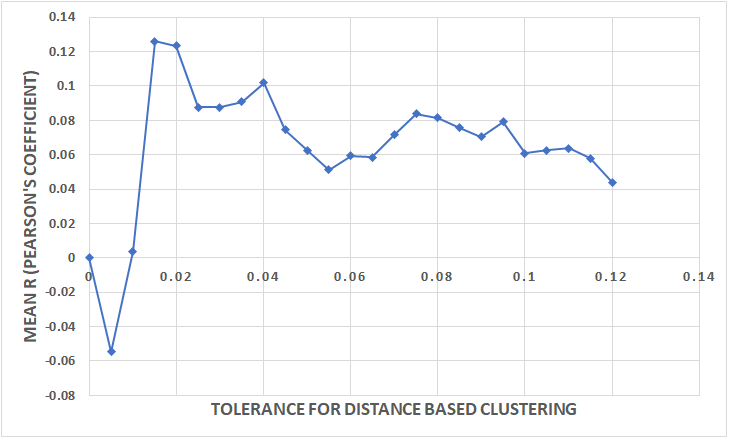
\includegraphics[width=400pt]{linegraph}
    \caption{\label{fig:linegraph} Pearson Coefficient vs Tolerance}
\end{figure}

\section{Challenges}

One of the challenges that faced while doing the analysis of the dataset was when the points are too far away from each other, this was because the units of one of the variable were really large. Since the parameter variable units were not comparable. The clustering algorithm was failing. Hence, to make it comparable the data was normalized. This normalization helped in making the parameters comparable. The tolerance was adjusted accordingly.

Another challenge faced was that because of normalization the real value of the slope got hidden. The normalization used was feature scaling the scales were changed and hence the slope and other values of the dataset did not correspond to what they should. To solve this problem, the dataset was then clustered using normalized value but the regression line was created for the raw values of the dataset. This help solves the clustering as well as the regression problem.
